\documentclass{article}
\usepackage[utf8]{inputenc}
%\usepackage[mathletters]{ucs}
\usepackage{lscape}
%\usepackage[utf8]{inputenc}
\usepackage[english]{babel}
%\usepackage[utf8]{inputenc}
%\usepackage{ucs}
%\usepackage[utf8x]{inputenc}
\usepackage{amsmath}

\usepackage{tikz}
\usetikzlibrary{positioning,shapes,fit,arrows, calc}

\usepackage{graphicx}
\usepackage[colorinlistoftodos]{todonotes}
\usepackage[ligature, inference]{semantic}
\usepackage{fixltx2e}
\usepackage{amsmath, listings, amsthm, amssymb, xspace}
\usepackage{amsmath}
\usepackage{inconsolata}
\usepackage{bussproofs}
\usepackage{mathpartir}
\usepackage[margin=0.5in]{geometry}
\usepackage{hyperref}
\usepackage{stmaryrd}
\hypersetup{
    colorlinks=true,
    linkcolor=blue,
    filecolor=magenta,      
    urlcolor=cyan,
}
\lstset{basicstyle=\tt}
\usepackage{unicode-math-defs}
\newtheorem{definition}{Definition}
\begin{document}

\title{Secure Typed Languages}
\author{Andrew Meyers}
\maketitle

\section*{Nondeterministic languages}

For nondeterminstic languages, the semantics does not just give one final state. We can define $\llbracket s \rrbracket$ to be a set of final states, or a distribution of states, or more exotically,  a mixture of distributions of states. The problem is then how to define noninterference $s_1 \sim_L s_2 \implies \llbracket s_1 \rrbracket \approx_L \llbracket s_2 \rrbracket$. The question is how to define $\approx_L$ for sets. 

[Sutherland '87] defined nondeducibility. The adversary sees a particular final state of the $s_1$ run, and we ask ourselves whether the result could have been produced by $s_2$. So we define 

\[
\llbracket s_1 \rrbracket \approx \llbracket s_2 \rrbracket = 
(\forall t_1 \in \llbracket s_1 \rrbracket \exists t_2 \in \llbracket s_2 \rrbracket . t_1 \sim_L t_2) \wedge (\forall t_2 \in \llbracket s_2 \rrbracket \exists t_1 \in \llbracket s_1 \rrbracket . t_2 \sim_L t_1)
\]

The following diagram illustrates this relationship.

  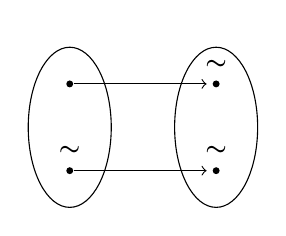
\begin{tikzpicture}
  [
      group/.style={ellipse, draw, minimum height=50pt, minimum width=30pt, label=above:#1},
      my dot/.style={circle, fill, minimum width=2.5pt, label=above:#1, inner sep=0pt}
    ]
    \node (a) [my dot=] {};
    \node (b) [below=of a, my dot=$\thicksim$] {};
    \node (c) [right=50pt of a, my dot=$\thicksim$] {};
    \node (d) [below=of c, my dot=$\thicksim$] {};
    \foreach \i/\j in {a/c,b/d}
      \draw [->, shorten >=2pt] (\i) -- (\j);
    \node [fit=(a) (b), group=] {};
    \node [fit=(c) (d) , group=] {};
  \end{tikzpicture}
\newline
This property can be enforced with the same type system as we saw last time. We can model nondeterminism with a nondeterministic choice construct $c_1 \Box c_2$. We can typecheck this language with the same rules. For integrity this is good enough but for confidentiality it is not. We give an example.

\[
pub := secret \Box put := rand(100)
\]

This is secure according to the previous definition of $\approx_L$ if $secret \in {0\dots 100}$, because for any one run we can't tell that secret has a particular value. Any number that is assigned to $pub$ could have been produced by the random number generator. However, if the adversary runs the program many times, it will be able to infer the value of secret because the probability that that value is produced is higher than the probability of the other numbers. Even if the adversary can only run the program once, the adversary still learns something in the information theoretic sense. Note that this is true even if the adversary does not control $\Box$.

The program has an insecure refinement $pub :=  secret$. This is called a refinement attack. Possibilistic security is not preserved under refinement. 

\section*{Low-security observational determinism (LSOD)}

Roscoe \cite{roscoe1995csp} proposed LSOD as a solution. Adversary-observable nondeterminism is subject to refinement attacks. We will require that execution looks deterministic from the point of view of the adversary:

\[
\llbracket s_1 \rrbracket \approx_L \llbracket s_2 \rrbracket = \forall t_1 \in \llbracket s_1 \rrbracket, t_2 \in \llbracket s_2 \rrbracket. t_1 \sim_L t_2
\]

One might think that this property is too restrictive for the programs that we want to write, because the following program is considered insecure:

\[put := true \Box put := false\]

This parallel program is also considered insecure:

\[put := true \parallel pub := false\]

We argue that these programs should be considered insecure. A secret could correlate with the nondeterminism, as in Meltdown and Spectre. 

Did we just lose the ability to write parallel programs at all? Consider the following program:

\[(x := 1 \parallel y := 2); \dots\]

This pattern is called fork-join parallelism. Two independent computations are done in parallel. Such harmless scheduling choices should be allowed. However, consider the following program:

\[ (x := true; \textbf{ if } h \textbf{ then } delay(100) \textbf{ else } skip; x := false)\text{ } \parallel (delay(50); \text{ } l := x)\]

This program is insecure, because the race between $x := false$ and $l := x$ allows an adversary to read the value of the secret $h$ using appropriate timing. This is called an internal timing channel. The program above converts the timing channel into a storage channel.

Assume that we have a trace $t = s,s',s'',\dots$, and assume that locations $m$ are a subset of the locations state. Let $t[m] = s[m],s'[m],s''[m],\dots$ be the projection of the state on the subset of the locations. We define $t_1 \sim_L t_2$ if the subtraces $t_1[m],t_2[m]$ are indistinguishable at $m$ modulo stuttering (collapse adjacent identical states of the subtraces to a single state). For termination insensitivity, if one trace is finite and the other trace is infinite, we only require them to agree up to the common prefix. 

\section*{Downgrading}

Requiring all information flow to obey the lattice order $\sqsubseteq$ is too restrictive.  Real applications need to be able to release secret information. The real security goal is not complete noninterference, but knowledge over how information can flow. We have two dual operations: (1) downgrading confidentiality: declassify(), and (2) downgrading integrity: endorse(). These are represented in the following lattice structure. For those unfamilar with lattice diagrams, it is noted that declassify suggests information flowing $H \sqsubseteq{} H^{\leftarrow{}}$, endorse suggests $L \sqsubseteq{} H^{\leftarrow{}}$, and that confidentiality increases as $\sqsubseteq{} H^{\rightarrow{}}$, and integrity as $\sqsubseteq{} H^{\leftarrow{}}$. This suggests that $L$ is potentially public, and to increase confidentiality does not always result in an increase in integrity. It is vital that data with a high confidentiality cannot be modified by data with low integrity, and in general, a secure system will require that no user with integrity less than the confidentiality can modify the data. 
\newline
%would add lattice here
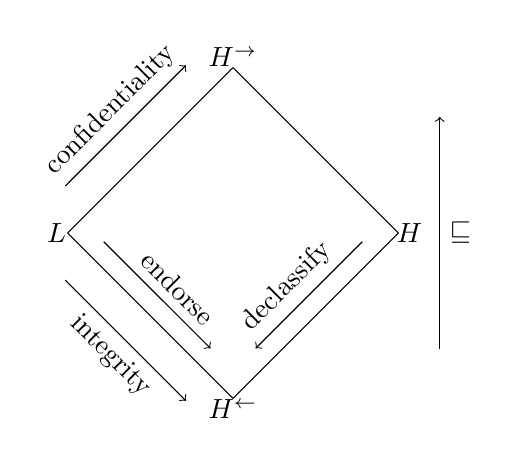
\begin{tikzpicture}[scale=.7]
  \node (one) at (0,3.2) {$H^{\rightarrow{}}$};
    \node(offsetone) at (3.75, 3){};
  \node (a) at (-3.2,0) {$L$};
  \node (d) at (3.2,0) {$H$};
  \node (zero) at (0,-3.2) {$H^{\leftarrow{}}$};
  \node(offset) at (3.75, -3){};
  \draw (0,-3)  -- (-3,0) ;
  \draw (0,3)  -- (-3,0) ;
  \draw (0,3)  -- (3,0);
  \draw (0,-3)  -- (3,0);
    \draw [shorten >=0.5cm,shorten <=.5cm,<-] (zero.225) -- (a.225) node [midway, below, sloped]  {integrity};
        \draw [shorten >=0.5cm,shorten <=.75cm,<-] (zero.45) -- (a.45) node [midway, above, sloped]  {endorse};
        \draw [shorten >=0.5cm,shorten <=.5cm,<-] (one.135) -- (a.135) node [midway, above, sloped]  {confidentiality};
         \draw [shorten >=0.5cm,shorten <=.75cm,<-] (zero.135) -- (d.135) node[ midway, above, sloped]  {declassify};
         \draw[shorten >=0.5cm, shorten <=.5cm, ->] (offset) -- (offsetone) node [midway, right]{$\sqsubseteq{}$};

\end{tikzpicture}
\newline
The justification for downgrading depends on the application, so we can't expect a type system to check this. We demonstrate this with a few examples. 

\subsection*{Example 1: Password Checker}

A password check will tell the user whether the password is correct, so the adversary learns something about the secret password:

\begin{lstlisting}[language=Java]
    if  (declassify(guess == password),H to L)) login = true;
\end{lstlisting}

\subsection*{Example 2: Battleship}

If player A makes a move, we check whether the move was legal, and then B applies the move to their copy of the board:

\begin{lstlisting}[language=Java]
    if(legal(mx,my)) endorse(mx,my)(A(<-) to B(<-))
\end{lstlisting}

The justification for the endorse lies in the rules of the game: A may choose any legal move, and then B must accept that move. In our lattice notation, this means that that if(legal (mx, my)) endorse (mx, my) ($A^{\leftarrow{}}$ to $B^{\leftarrow{}}$, then we apply move to B's copy of the board. E.g, (mx, my):$A^{\leftarrow{}}$. We demonstrate this in the below diagram.
\newline
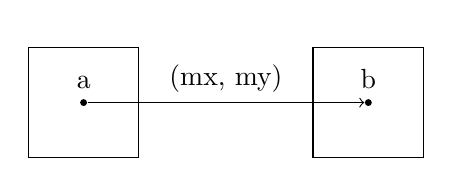
\begin{tikzpicture}
  [
      group/.style={rectangle, draw, minimum height=40pt, minimum width=40pt, label=above:#1},
      my dot/.style={circle, fill, minimum width=2.5pt, label=above:#1, inner sep=0pt},
      dotty/.style={ label=above:#1},
    ]
  
    \node (a)  [my dot=a] at (0,5) {};

    \node (c) [right=100pt of a, my dot=b] {};

      \draw [->] (a) -- (c) node [midway, above] {(mx, my) };
    \node [fit=(a), group=] {};
    \node[ fit=(c), group=]{};

  \end{tikzpicture}

\subsection*{Example 3: average of a set of confidential salaries}

We can compute the average of a set of secret salaries and add random noise to make sure that we do not provide too much information about anys individual salary.

\begin{lstlisting}[language=Java]
    float arg = declassify(mean(salaries) + noise, H^-> to L)
\end{lstlisting}

The justification for the declassify comes from differential privacy.

With downgrading we no longer have noninterference:

\begin{lstlisting}[language=Java]
    string{H} 
    bool{L} check(string {H} guess) {
        return declassify(guess == pwd, ...)
    }
\end{lstlisting}

The label H represents confidentiality. The adversary can overwrite the password with a secret, and then test that secret against a guess, thus leaking secret information. This is called laundering secrets via declassify.

This example shows that we need sufficient integrity to securely declassify - we need to ensure that the adversary can't affect what is declassified or whether something is declassified.

Implementations of this are a message passing concurrent language based on the join calculus [1], Chong et al. [2], JOANA [3].
\cite{zdancewic2003observational}

\subsection*{Robust declassification}

Robust declassification (Zdancewic \cite{zdancewic2001robust}) is a solution to the problem of secure declassifcation.
We define the view operator, which defines the confidentiality level such that the integrity of $pc, l$ are both trusted to declassify. 

\[
\inference{l_2 \sqsubseteq{} \Gamma(x) ~~~~~ \Gamma(y) \sqsubseteq{} l_1 ~~~~~ l_1 \sqsubseteq{} l_2 \sqcup \bigtriangleup (l_1 \sqcup pc) }{pc \vdash x:= \texttt{declassify}(y, l_1 \texttt{ to } l_2) }
\]
The following lattice diagram demonstrates this relationship, as does the mapping of relationships between labels. The shaded region suggests "unsafe" regions and flows, where a secure system should not allow modification or access. \newline
%The following lattice diagram demonstrates this. \\
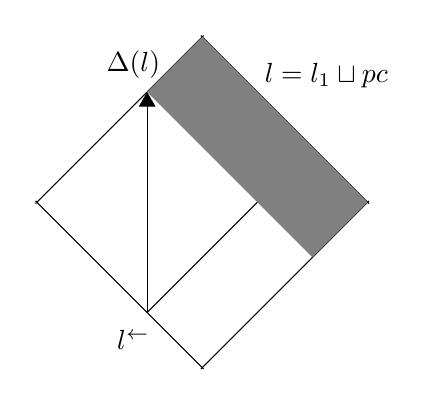
\begin{tikzpicture}[scale=.7]
  \node (one) at (0,3) {};

  \node (a) at (-3,0) {};
\node (aoff) at (-1.25,2.50) {$\Delta(l)$};
  \node (d) at (3,0) {};
  \node (doff) at (-1.25,-2.5) {$l^{\leftarrow{}}$};
    \node (doffleft) at (2.25,2.30) {$l=l_1\sqcup pc$};
     \node (doffsouth) at (2.25,-1.60) {};
  \node (zero) at (0,-3) {};

  \node(offset) at (3.5, -2){};
  \draw[shorten >=-.20cm, shorten <=-.2cm] (zero) -- (a);
  \draw[shorten >=-.20cm, shorten <=-.2cm] (one) -- (a);
  \draw[shorten >=-.20cm, shorten <=-.2cm] (one) -- (d);
  \draw[shorten >=-.20cm, shorten <=-.2cm] (zero) -- (d);
  \draw[>= triangle 60, <-] (-1,2) -- (-1,-2) ;

  \draw (2,1.0) -- (-1,-2);
% \draw[shorten >=-.25cm, shorten <=-.05cm]  (aoff) -- (doffsouth);
  
  \path[fill, color=gray] (-1,2) --(2,-1) --  (3,0)-- (0,3) ;

\end{tikzpicture}
\hspace{2cm}
  \raisebox{4em}{ 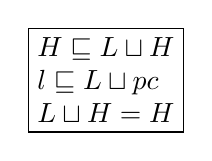
\begin{tikzpicture}
    \node[draw,align=left] {$H\sqsubseteq{} L \sqcup H$\\
$l\sqsubseteq{} L \sqcup pc$\\
$L\sqcup H=H$};
  \end{tikzpicture}
  }
\hspace{2cm}
  \raisebox{3em}{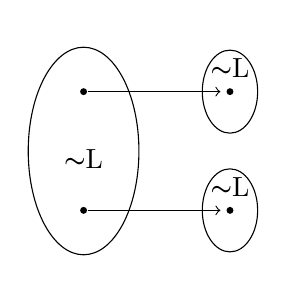
\begin{tikzpicture}
  [
      group/.style={ellipse, draw, minimum height=75pt, minimum width=40pt, label=above:#1},
      groupsm/.style={ellipse, draw, minimum height=30pt, minimum width=20pt, label=above:#1},
      my dot/.style={circle, fill, minimum width=2.5pt, label=above:#1, inner sep=0pt},
      dotty/.style={ label=above:#1},
    ]
  
    \node (a)  [my dot=] at (0,5) {};
    \node(e) [below=30pt of a,  dotty=$\thicksim$L] {};
    \node (b) [below=40pt of a, my dot=] {};
    \node (c) [right=50pt of a, my dot=$\thicksim$L] {};
    \node (d) [below=40pt of c, my dot=$\thicksim$L] {};
    \foreach \i/\j in {a/c,b/d}
      \draw [->, shorten >=2pt] (\i) -- (\j);
    \node [fit=(a) (b), group=] {};
    \node [fit=(c) , groupsm=] {};
     \node [fit=(d) , groupsm=] {};
  \end{tikzpicture}
  }
\newline
%Add the other diagram of circles
Robust declassification thus implies that the adversary cannot increase leakage. Leakage will exist, but the adversary cannot increase the amount of information leaked.
We define $s[a]$ is defined as the state with an attack $a$ applied to it. $a$ must be a fair attack, it cannot just violate noninterference randomly.  Furthermore, it must typecheck within the $pc$ corresponding to $L$
 The formal definition of robust declassification semantics is as follows:

\[
\forall s,s',a,a'. \text{ relevant attack } (a) \wedge s[a] \approx_L s'[a] \implies s[a'] \approx_L s'[a']
\]




We summarize the number of traces we have to compare to establish each corresponding property in a table.

\begin{table}[h]
\begin{tabular}{|l|l|l|}
\hline
Method & Traces\\
\hline 
 Correctness & 1 trace \\\hline
 Noninterference, LSOD & 2 traces \\ \hline
 Robust declassification & 4 traces \\ \hline
\end{tabular}
\end{table}

For those interested in learning more check out the following references: 

For a message passing concurrent language see
\cite{zdancewic2003observational}

The X10 programming language implemented some of these ideas.
\cite{charles2005x10}

Java Object-sensitive ANAlysis (JOANA) \cite{milanova2005parameterized}

\bibliographystyle{unsrt}
\bibliography{bib2}
\end{document}
